\documentclass{article}

% Configurações Genéricas ------------------------------------------------------
\usepackage[utf8]{inputenc}
\usepackage[T1]{fontenc}
\usepackage[brazil]{babel}
\usepackage{sbc-template}
\usepackage{graphicx}

% Informações Pessoais ---------------------------------------------------------
\title{Tarefa 02 sobre Desenvolvimento com J2ME}
\author{Wanderson Henrique Camargo Rosa\inst{1}}
\address{Programação para Dispositivos Móveis 2011/1\\Centro de Ciências Exatas
e Tecnológicas\\Universidade do Vale do Rio dos Sinos ---
UNISINOS\email{wandersonwhcr@gmail.com}}

% Documento --------------------------------------------------------------------
\begin{document}

\maketitle{}

% Introdução -------------------------------------------------------------------
\section{Introdução}
\label{sec:introducao}

Conforme tarefa da segunda semana da disciplina de Programação para Dispositivos
Móveis, existe a necessidade de criação de um aplicativo simples que deve ser
executada no simulador. Para documentação, deve-se gerar um relatório de
atividade relatando os passos realizados.

O presente documento é resultado final desta tarefa e busca relatar sobre os
serviços executados durante o desenvolvimento do \emph{software}.

% Instalação do Ambiente -------------------------------------------------------
\section{Instalação do Ambiente}
\label{sec:instalacao}

O ambiente de desenvolvimento escolhido foi Eclipse, plataforma que já utilizo
em outras áreas de desenvolvimento. Visitando a página de \emph{download}, a
primeira idéia que sempre tive foi que o JavaEE seria o ambiente para criação de
aplicativos para dispositivos móveis, o que foi brevemente foi retirado quando
li alguns textos sobre.

Resolvi copiar a versão para desenvolvimento em Java. Logo após, procurei
informações sobre como desenvolver aplicativos J2ME no ambiente. Encontrei o
\emph{plugin} MTJ, sucessor do EclipseME. O gerenciamento de pacotes do projeto
MTJ traz alguns problemas quanto a atualização entre versões, o que é impossível
porque o endereço URL é fixo para cada versão. Após instalar a última versão,
tentei gerar um novo projeto, sem sucesso.

Para criação deste é necessário um dispositivo para emulação que não estava
instalado. Eu particularmente achava que eles já teriam sido instalados junto
com o \emph{plugin}. Após compreender o problema, resolvi ler a documentação
disponível na tarefa e encontrei a WDK. Para instalação, a WDK exige o diretório
onde a máquina virtual Java está instalada. O Ubuntu salva este diretório em um
local diferenciado, possivelmente visando velocidade.

O Eclipse necessita de configurações para encontrar o caminho da WDK e o caminho
para pesquisa de dispositivos para emulação. Após o fornecimentos destas
informações, o Eclipse exibe 4 dispositivos encontrados.

\subsection{Problemas com Arquitetura}

Seguindo o \emph{tutorial} fornecido na documentação da disciplina, não consegui
diretamente executar o aplicativo proposto, gerando um erro de tamanho de
palavra. Após algum tempo de pesquisa, percebi que a arquitetura do WTK
somente estava disponível em 32 bits e o ambiente Eclipse utilizado é 64 bits.

Portanto, tive que instalar todo o ambiente novamente, porém buscando os
executáveis no formato 32 bits. Após, o desenvolvimento da aplicação proposta
pelo \emph{tutorial} foi finalizado e finalmente tive oportunidade de idealizar
o desenvolvimento da tarefa 02.

% Sobre o Aplicativo -----------------------------------------------------------
\section{Sobre o Aplicativo}
\label{sec:sobre}

Conforme primeira aula presencial da disciplina, o J2ME receberá uma atenção
menor porque está sendo menos usado hoje em dia. Outras tecnologias serão
inseridas no conteúdo com o passar das aulas. Porém, nesta semana, devemos criar
uma aplicação simples.

\subsection{Apresentador de \emph{Slides}}

A primeira idéia de desenvolvimento foi um aplicativo que estou idealizando para
Android há quase 1 ano. Um apresentador de \emph{slides} é um dispositivo de
\emph{hardware} que trabalha como um controle remoto para navegação em exibição
de palestras. O problema é que este dispositivo custa muito caro pelas funções
que executa.

Basicamente, precisamos de um elemento que estabeleça uma conexão com o
computador da apresentação e envie comandos para avançar ou retroceder
\emph{slides}. Um dispositivo móvel como um celular \emph{smartphone} possui
estas características e pode receber um programa capaz de abranger as
necessidades.

Para troca de informações com o computador, devemos criar um programa servidor
que administre conexões e interprete os comandos enviados pelo dispositivo
móvel.

Como esta tarefa é um pouco maior e a idéia principal do desenvolvimento sobre
J2ME não deve ser tão complexa, resolvi deixar este para aplicar sobre a
plataforma Android, próximo assunto da disciplina.

\subsection{Desenho Simples}

A segunda tarefa da disciplina está focada no desenvolvimento de um aplicativo
simples. Basicamente, um programa J2ME deste tipo pode, além de iniciar
corretamente, possuir:

\begin{itemize}
  \item Entrada e saída de informações;
  \item Manipulação dos dados fornecidos; e
  \item Utilização dos componentes disponíveis.
\end{itemize}

Assim, desenvolvi um programa que possui um ambiente para desenho muito simples,
onde o usuário pode movimentar o cursor e colorir a localização atual do mesmo,
chamado JDrawME.

% JDrawME ----------------------------------------------------------------------
\section{JDrawME}
\label{sec:jdrawme}

O JDrawME é um aplicativo que carrega uma tela da cor preta na tela e cria um
cursor branco que pode ser movimentado utilizando os números do teclado. A
posição atual do cursor pode ser colorida através de um número específico. Para
finalização, há um comando para saída.

\begin{figure}
    \centering{}
    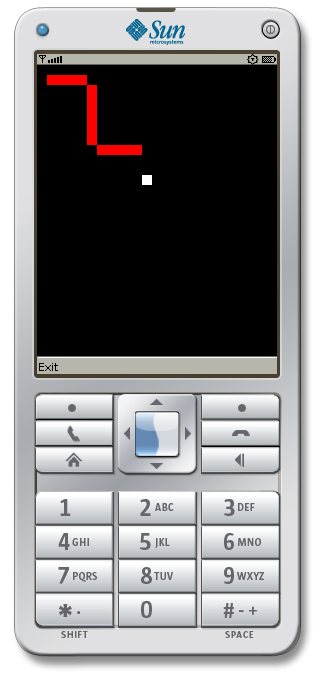
\includegraphics[scale=0.4]{screenshot01-emulator.png}
    \caption{Captura de Tela do Emulador}
    \label{fig:emulador}
\end{figure}

Podemos visualizar uma captura de tela do JDrawME sendo executado no emulador na
Figura \ref{fig:emulador}.

\subsection{Teclas para Movimentação e Desenho}

O cursor pode ser movimentado e a posição colorida utilizando as seguintes
teclas:

\begin{description}
\item[Número 2] Movimenta o cursor para cima;
\item[Número 8] Movimenta o cursor para baixo;
\item[Número 4] Movimenta o cursor para esquerda;
\item[Número 6] Movimenta o cursor para direita; e
\item[Número 5] Colore a posição atual do cursor.
\end{description}

\subsection{Classes}

Buscando dividir as tarefas, criei algumas classes para encapsulamento de
funcionalidades. A estrutura do projeto pode ser visualizada na Figura
\ref{fig:projeto}.

\begin{figure}
    \centering{}
    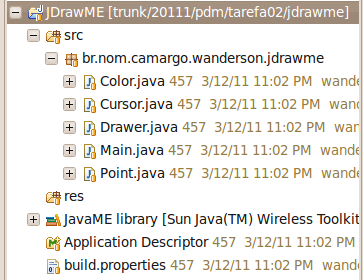
\includegraphics[scale=0.45]{screenshot01-project.png}
    \caption{Estrutura do Projeto}
    \label{fig:projeto}
\end{figure}

A classe \texttt{Main} é responsável pela execução principal do programa que
inicializa um objeto da classe \texttt{Drawer}, estendida da classe
\texttt{Canvas}, que recebe o controle de desenho. Houve a necessidade de
criação da classe \texttt{Point} para trabalhar como pontos em tela e sua
derivada \texttt{Cursor} para controlar a movimentação. Finalizando, existe a
classe \texttt{Color} que administra a manipulação de cores.

\subsection{Funcionalidades}

Os principais métodos da aplicação são duas sobrescritas da classe
\texttt{Canvas} na \texttt{Drawer}, uma para controle de pintura em tela e
outra que administra os pontos já inseridos.

Quando uma tecla é pressionada, o método \texttt{keyPressed} é chamado pelo
Java. Um bloco condicional do tipo \texttt{switch} foi desenvolvido e as
chamadas de movimentação são delegadas para cada tecla. Caso a tecla de
colorização seja ativada, um novo cursor é adicionado a uma lista de objetos
pertencente ao objeto do tipo \texttt{Drawer}. Ao final, solicita-se que o
ambiente seja redesenhado.

Neste momento, o Java executa o método \texttt{paint}, que limpa o ambiente de
desenho com a cor de fundo configurada, renderiza cada ponto adicionado à lista
com a cor de primeiro plano. Ao final, o cursor é renderizado com cor inversa ao
fundo na posição atual.

\subsection{Execução}

Após gerar o MIDlet, executei em duas plataformas: uma emulada do próprio WTK e
um celular Nokia C3-00 com sistema operacional Nokia S40 Mobile, conforme
Figura \ref{fig:nokia}. Por ser muito simples, nenhuma arquitetura ocasionou
defeito, porém no celular físico a tecla SHIFT precisa ser pressionada para
acessar os números.

\begin{figure}
    \centering{}
    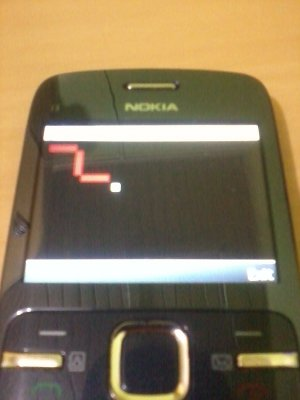
\includegraphics[scale=0.5]{screenshot02.jpg}
    \caption{Aplicativo Executado no Nokia C3-00}
    \label{fig:nokia}
\end{figure}

% Anotações Finais -------------------------------------------------------------
\section{Anotações Finais}
\label{sec:finais}

A facilidade de desenvolvimento sobre a plataforma J2ME é muito visível quando o
programador está acostumado com o ambiente Java. Podemos concluir que existem
diferenças nos componentes utilizados, porém a lógica de aplicação é a mesma.

Senti dificuldades na pesquisa de estruturas de dados disponíveis. O Java para
\emph{desktops} possui uma grande de quantidades de listas encadeadas
disponíveis. Para J2ME somente encontrei uma implementação da classe
\texttt{Vector}.

Também encontrei diferença quanto a utilização do laço de repetição
\texttt{for}. Este não pode ser utilizado com um elemento anônimo para iteração
com todos os objetos inclusos em uma lista. Isto deve acontecer para otimização
da máquina virtual que é executada sobre dispositivos embarcados.

A portabilidade do Java sobre as plataformas embarcadas é dificultada quando
dispositivos diferentes recebem o programa. Podemos exemplificar com a execução
do mesmo aplicativo sobre o emulador com teclado de dígitos e o celular com
teclado completo e sem acesso direto aos números, ou com o tamanho da tela que
no emulador possui orientação vertical e no celular orientação horizontal.

O programador deve especificar arquiteturas semelhantes para execução do
programa ou tratar todas as possibilidades de entrada e saída, algo quase
impossível se comparado com a quantidade de dispositivos que possuem uma máquina
virtual Java.

Para a instalação do ambiente de desenvolvimento foram gastos 3h30min, a
inicialização no desenvolvimento, ambientação com a linguagem e estrutura e
aplicação dos \emph{tutoriais} fornecidos ocorreu em 2h, aprendizado sobre
componentes disponibilizados pelo J2ME em 2h, desenvolvimento do aplicativo
final em 4h30min e documentação final em cerca de 4h. Todos estes horários somam
16h estão distribuídos entre os dias 09 de março e 13 de março de 2011.

Fico com idéias para desenvolvimento com a próxima plataforma de estudo da
disciplina, um apresentador de \emph{slides} para Android.

\end{document}